\documentclass[11pt]{article}

\usepackage[utf8]{inputenc}
\usepackage[T1]{fontenc}
\usepackage{lmodern}
\usepackage{amsmath,amsfonts}
\usepackage{subfigure}
\usepackage{bm}
\usepackage{listings}
\usepackage{pifont}%
\usepackage{xcolor}

\usepackage{pgfplots,tikz}

\usepackage{fullpage}      % Margens
\usepackage{indentfirst}   % Autoidentar
\usepackage{graphicx}       % Pictures

\newcommand{\answer}[1]{\color{blue}{#1}\color{black}}

\begin{document}

\noindent Northeastern University
\hfill March 26, 2018

\noindent Department of Electrical and Computer Engineering
\hfill EECE5698-ST (Spring 2018)

\noindent {} \hfill \textbf{Homework 3}

\noindent \rule{\linewidth}{1.5pt}

\vspace*{.5cm}

\underline{Due date}: Wednesday 4, April 2018. Hand in at class or send a scanned copy to closas@northeastern.edu

To complete the problems, feel free to consult other sources (i.e., books, internet, etc.) besides class notes.  Justify your answers!

\noindent \rule{\linewidth}{1pt}
\vspace*{1cm}


% \textbf{Problem}:
Taking as a reference the WLSA algorithm (implemented in HW2), implement a Kalman filter solution as the positioning algorithm. 
Similarly as in WLSA (and WLS), initialize variables and replicate error computation and plotting code.

Recall that in the KF solution, the a priori information, comes from the previous state estimate, $\hat{\mathbf{x}}_{t-1|t-1}$, with covariance matrix $\mathbf{P}_{t-1|t-1}$. These are computed sequentially

\begin{enumerate}
\item[(a)] Given that $\mathbf{x}$ includes position ($\mathbf{p}$) and clock offset ($c \delta t$), define suitable values for the mean and covariance of the initial information given to the KF
\begin{equation}
\nonumber \mathbf{x}_{0|0} \sim \mathcal{N}(\hat{\mathbf{x}}_{0|0},\mathbf{P}_{0|0}) \;,
\end{equation}
\noindent if we would like to inform the algorithm that the receiver is somewhere in $i)$ USA, and $ii)$ Boston. Recall that initial values (and thus a priori) are defined in ECEF.

\answer{
In the last homework, we found mean positions and covariance matrices based respectively on the geographic centers and dimensions of the USA, Massachusetts and Boston to use as priors for the WLSA algorithm. These priors can be used as the initial state $\mathbf{x}_{0|0}$ and state covariance $\mathbf{P}_{t-1|t-1}$ for the Kalman algorithm as well.

For the United States, in ECEF coordinates, these are:

\[
   x =
  \left[ {\begin{array}{c}
   -0.7321 * 10^6 \\
   -4.8502 * 10^6 \\
   4.0640 * 10^6 \\
   0 \\
  \end{array} } \right], 
  %
   P=
  \left[ {\begin{array}{cccc}
   [2546*10^3 & 0 & 0 & 0 \\
   0 & 4313*10^3 & 0 & 0 \\
   0 & 0 & 50 & 0 \\
   0 & 0 & 0 & 10^5 \\
  \end{array} } \right]
\]

For Boston, in ECEF coordinates, these are:

\[
   x =
  \left[ {\begin{array}{c}
   1.5322 * 10^6 \\
   -4.4646 * 10^6 \\
   4.2751 * 10^6 \\
   0 \\
  \end{array} } \right], 
  %
   P =
  \left[ {\begin{array}{cccc}
   67820 & 0 & 0 & 0 \\
   0 & 67820 & 0 & 0 \\
   0 & 0 & 50 & 0 \\
   0 & 0 & 0 & 10^5 \\
  \end{array} } \right]
\]

}

\item[(b)] Under the assumption that the receiver is static, what is a reasonable choice for the transition matrix $\mathbf{F}$ and process covariance matrix $\mathbf{Q}$?

\answer{
Under the assumption that the receiver is static, we would not expect the state to change from time t to t+1. Therefore, the most suitable choice for the tranition matrix is identity.

The process noise covariance is a bit less obvious, but if we assume that the true position of the receiver stays within 10m of its intended location, then we can define the first 3 elements of the diagonal as 10m, 10m and 10m respectively. The variance of the clock offset was determined through trial and error, and it was found that the Kalman filter performed better with a clock offset variance of about 10^5.

\[
   F=
  \left[ {\begin{array}{cccc}
   1 & 0 & 0 & 0 \\
   0 & 1 & 0 & 0 \\
   0 & 0 & 1 & 0 \\
   0 & 0 & 0 & 1 \\
  \end{array} } \right], 
  %
   Q=
  \left[ {\begin{array}{cccc}
   10 & 0 & 0 & 0 \\
   0 & 10 & 0 & 0 \\
   0 & 0 & 10 & 0 \\
   0 & 0 & 0 & 10^5 \\
  \end{array} } \right]
\]

}

\item[(c)] If the receiver has dynamics, what could be a better choice for $\mathbf{F}$ and $\mathbf{Q}$? if, to account for such dynamics, we would like to augment $\mathbf{x}$ to include the three-dimensional velocity coordinates $\mathbf{v}$, how should we modify $\mathbf{F}$ and $\mathbf{Q}$? 

\answer{
If we augment the state vector with velocity, our state becomes a 7-element vector. Thus, we expect our F and Q matrices to each be 7x7. Given this state definition, and the kinematics of free space, the states for the position of the receiver at time t+1 will be given by the sum of the position at time t, plus the velocity at time t multiplied by the duration of the interval between updates $\Delta T$.

If we define our state in the following way

\[
   x =
  \left[ {\begin{array}{c}
   p_x \\
   p_y \\
   p_z \\
   v_x \\
   v_y \\
   v_z \\
   c \delta t \\
  \end{array} } \right]
  
\]

then the state transition matrix which represents these kinematics is

\[
   F =
   \left[ {\begin{array}{ccccccc}
    1 & 0 & 0 & \Delta T & 0 & 0 & 0 \\
    0 & 1 & 0 & 0 & \Delta T & 0 & 0 \\
    0 & 0 & 1 & 0 & 0 & \Delta T & 0 \\
    0 & 0 & 0 & 1 & 0 & 0 & 0 \\
    0 & 0 & 0 & 0 & 1 & 0 & 0 \\
    0 & 0 & 0 & 0 & 0 & 1 & 0 \\
    0 & 0 & 0 & 0 & 0 & 0 & 1 \\
  \end{array} } \right]
  
\]

Under the assumption that the velocities in each of the dimensions are mutually independent of all other states, and each have variance of 10m/s, the process noise covariance matrix is

\[
   Q =
   \left[ {\begin{array}{ccccccc}
    10 & 0 & 0 & 0 & 0 & 0 & 0 \\
    0 & 10 & 0 & 0 & 0 & 0 & 0 \\
    0 & 0 & 10 & 0 & 0 & 0 & 0 \\
    0 & 0 & 0 & 10 & 0 & 0 & 0 \\
    0 & 0 & 0 & 0 & 10 & 0 & 0 \\
    0 & 0 & 0 & 0 & 0 & 10 & 0 \\
    0 & 0 & 0 & 0 & 0 & 0 & 10^5 \\
  \end{array} } \right]
  
\]

}

\end{enumerate}




Under the assumption that the receiver is static, implement the KF and test it with the initialization conditions in (a).
\begin{enumerate}
\item[(d)] Plot the error $\mathbf{e}_t = \mathbf{p}_t - \hat{\mathbf{p}}_t$ in the three coordinates over time. Is it decreasing or increasing?

\answer{

\begin{figure*}[ht]
    \centering
    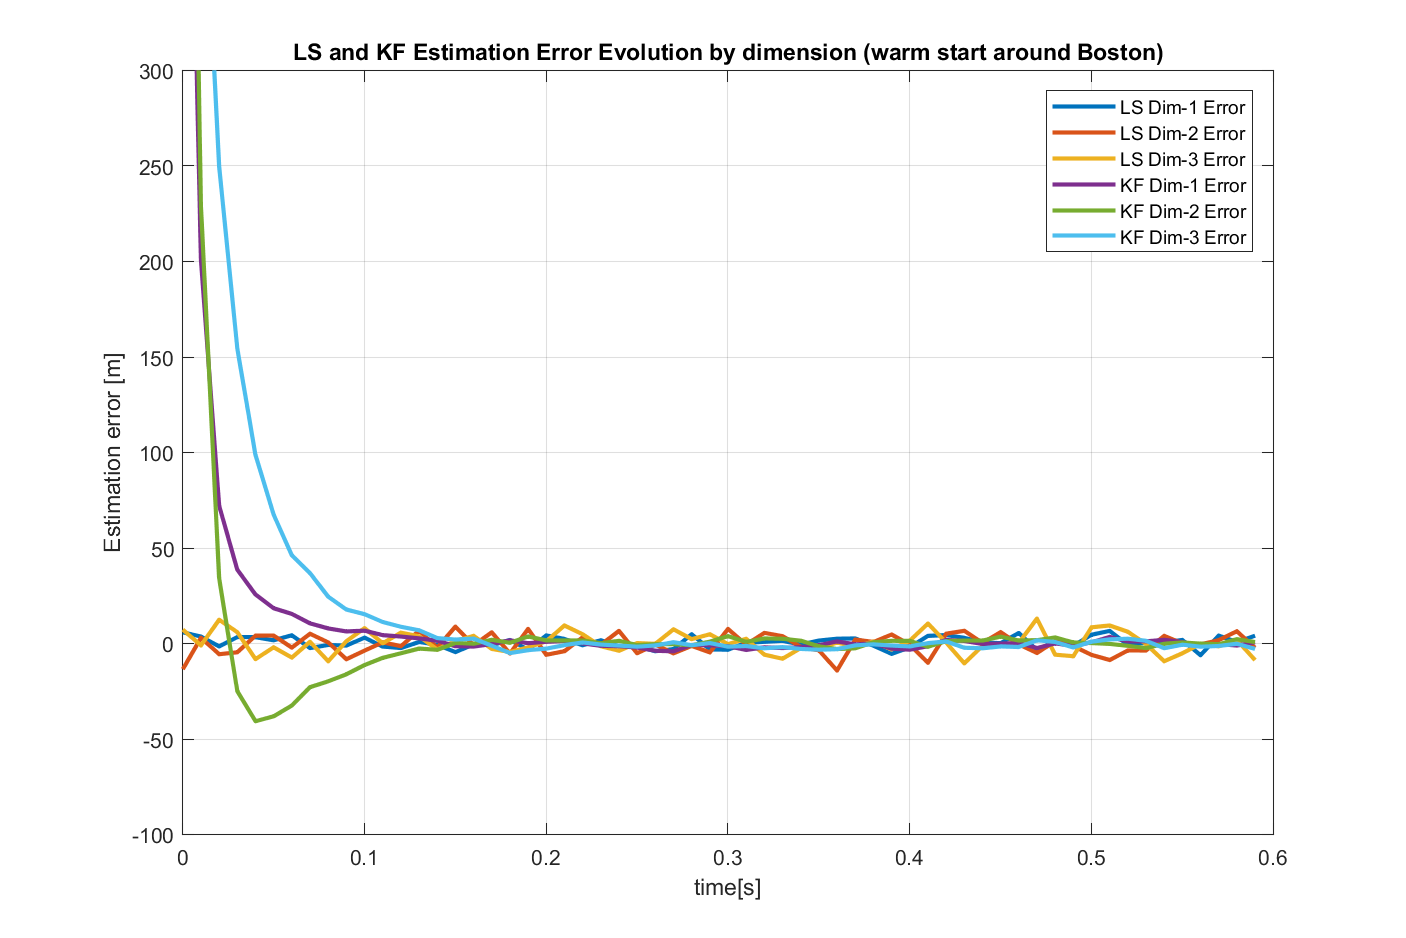
\includegraphics[width=0.8\textwidth]{HW3/latex/figures/ErrBoston.png}
    \caption{Time evolution of Least Squares and Kalman filter estimation error given a warm start defined by the initial state $\mathbf{x}_{0|0}$ and state covariance $\mathbf{P}_{t-1|t-1}$ for Boston described in part (a)}
    \label{fig:ErrBoston}
\end{figure*}

Figure \ref{fig:ErrBoston} shows that the Kalman estimation error decreases over time, and converges on the true position at about the 0.15 second mark.

\begin{figure*}[ht]
    \centering
    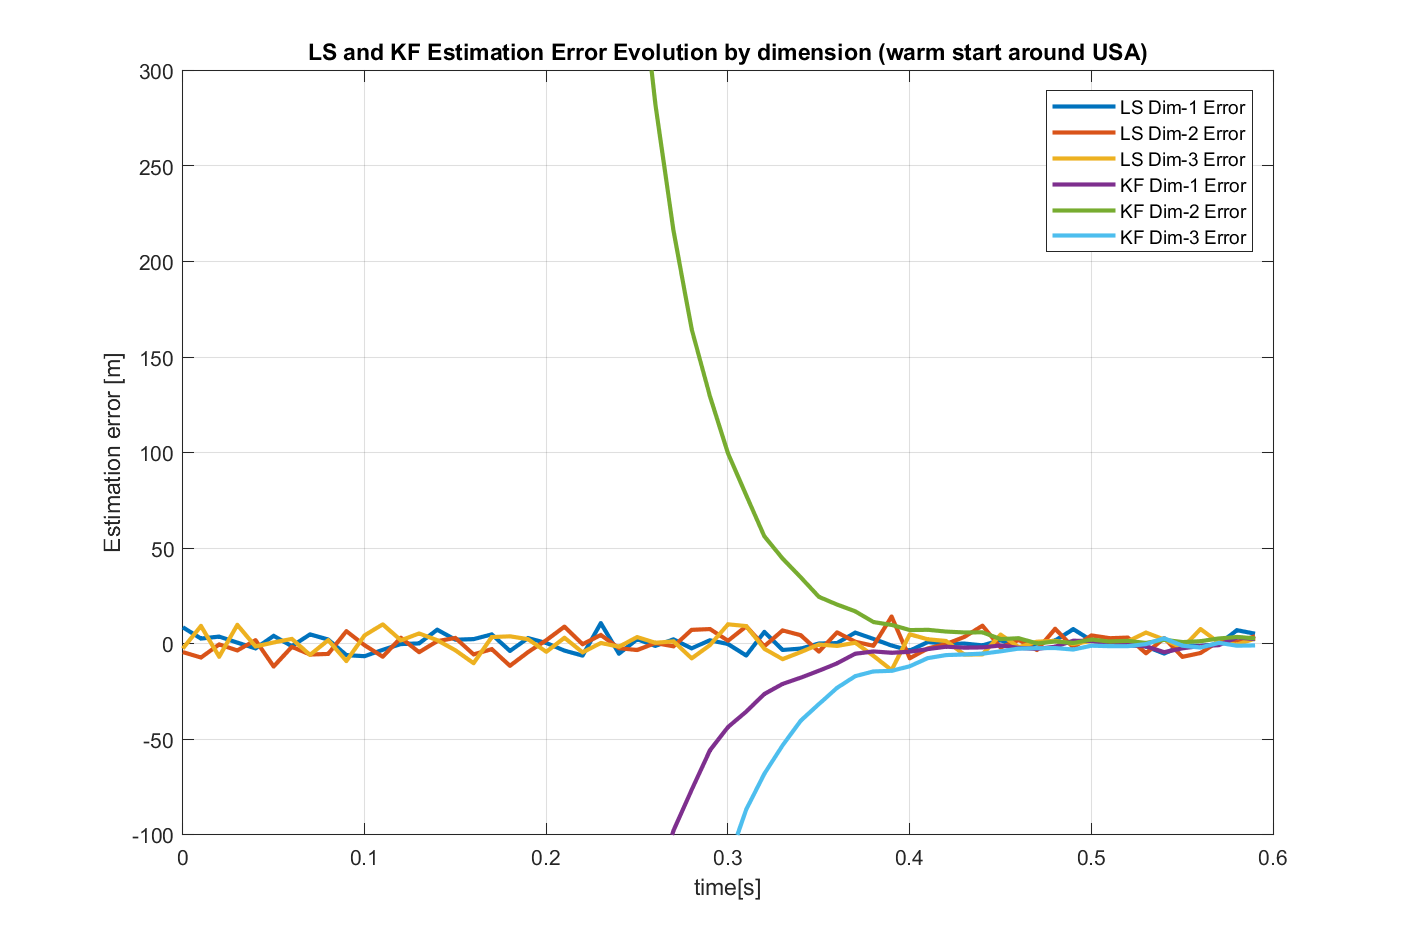
\includegraphics[width=0.8\textwidth]{HW3/latex/figures/ErrUSA.png}
    \caption{Time evolution of Least Squares and Kalman filter estimation error given a warm start defined by the initial state $\mathbf{x}_{0|0}$ and state covariance $\mathbf{P}_{t-1|t-1}$ for USA described in part (a)}
    \label{fig:ErrUSA}
\end{figure*}

By comparison, Figure \ref{fig:ErrUSA} shows the error for a warm start around the geographic center of the United States. It can be seen that while the Kalman algorithm still converges to the true position, it takes longer given a less informative initial prior.

}

\item[(e)] Compare $\mathbf{e}_t$ obtained with the KF and that obtained using LS or WLS solutions. Comment.

\answer{

Comparing the behavior shown in Figure \ref{fig:ErrBoston} for the LS and KF algorithms respectively, it's clear that the LS algorithm converges to the true location faster than the KF algorithm. We expect this to be the case under static conditions, but we expect that the Kalman filter will do a better job of tracking the position of the reciever under dynamic conditions. 

}

\item[(f)] Plot over time the elements of the covariance matrix ($\mathbf{P}_{t|t}$) relevant to $\mathbf{p}_t$. Are the obtained results coherent with those in (d)?

\answer{

\begin{figure*}[ht]
    \centering
    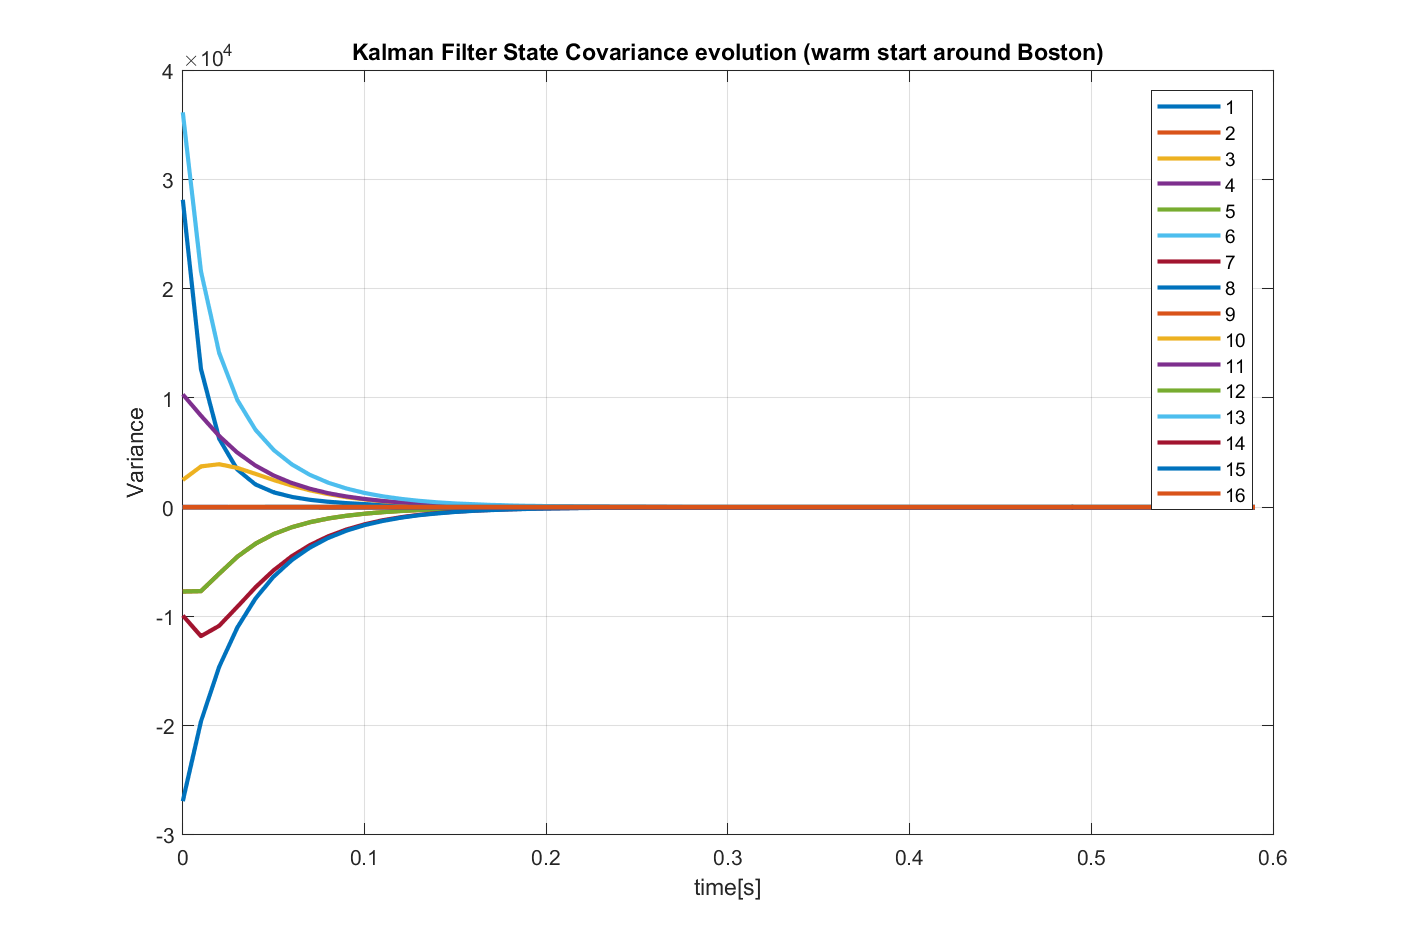
\includegraphics[width=0.8\textwidth]{HW3/latex/figures/CovBoston.png}
    \caption{Time evolution of Kalman filter state covariance given a warm start defined by the initial state $\mathbf{x}_{0|0}$ and state covariance $\mathbf{P}_{t-1|t-1}$ for USA described in part (a)}
    \label{fig:CovBoston}
\end{figure*}

Figure \ref{fig:CovBoston} shows the evolution of the elements of the state covariance matrix over time. These results are consistent with the results obtained in (d). As we would expect, as the Kalman estimate converges on the true location of the receiver the elements of the state covariance converge to zero.

}
\end{enumerate}


Hint: use the KF formulation in the slides, where unknown variables are already position and clock offset. Proceed similarly as for the WLSA in terms of defining variables in the main script. Additionally, you'll need to define the a priori parameters in the script and feed them to \verb|GNSS_KF_position.m|



\end{document}